\documentclass{siproblemset}

% SI Session Information
\course{MTH 1321}       % the course of your SI
\sessionnum{9}          % (optional) specify the session number
\sessiondate{3/2/21}   % the date of the session

\warmup{Concept Review}
\topic{Rates of Change}
\topic{Higher Derivatives}
\topic{Trigonometric Derivatives}
\cooldown{Graphs of Derivatives}

% Worksheet Information
\title{Rates of Change, Trig.\linebreak and Higher Derivatives}
\sections{Sections 3.4 and 3.5}
\withnamespace

\begin{document}
    \maketitle
    
    \activity{Warmup}{Concept Review}{Try these problems \textbf{alone} as your peers join the session. Do your best to not refer to your notes.}{15 minutes}

    \frq{What is the mathematical relationship between position, velocity, acceleration, and speed?}
    \smallspace
    \mcq[2]{Give the following derivatives.}{
        \task $\dddx\sin(x)=$
        \tinysp
        \task $\dddx\cos(x)=$
        \task $\dddx\sec(x)=$
        \tinysp
        \task $\dddx\csc(x)=$
        \task $\dddx\tan(x)=$
        \tinysp
        \task $\dddx\cot(x)=$
    }
    \frq{What is the derivative of $f(x)=-\sec(x)\cot(x)$?}
    
    \pagebreak
    \activity{Activity 1}{Rates of Change}{Work together in your \textbf{breakout rooms} to answer these questions. Do your best to not refer to your notes while working on these problems.}{30 minutes}
    
    \mcq{A ball is thrown upwards off of the roof of a building on an extraterrestrial planet. The height of the ball (in meters) at time $t$ (in seconds) is given by $$s(t)=200+7t-4t^2$$}{
        \task What is the height of the building?
        \normalsp
        \task What was the initial velocity of the ball?
        \normalsp
        \task When will the ball hit the ground?
        \normalsp
        \task How fast is the ball going when it hits the ground?
        \normalsp
        \task What is the acceleration due to gravity on this planet?
        \normalsp
    }
    \frq{The tangent lines to the graph $f(x)=\sec(x)$ grow steeper as $x$ increases. At what rate do the slopes of the tangent lines increase?}
    \mediumspace
    
    \pagebreak
    
    \activity{Activity 2}{Higher-Order Derivatives}{Work together in your \textbf{breakout rooms} to answer these questions. Do your best to not refer to your notes while working on these problems.}{30 minutes}
    
    \mcq{Find $f'(x)$, $f''(x)$, and $f'''(x)$.}{
        \task{$f(x)=2x^3-3x^2+2x-\cos(x)$}
        \mediumspace
        \task{$f(x)=3e^x-x^3$}
        \mediumspace
        \task{$f(x)=\dfrac{1}{x}$}
        \mediumspace
        \task{$f(x)=(2x+1)(x^2-2)$}
        \mediumspace
        \task{$f(x)=\pi^2(x-1)$}
        \mediumspace
        \task{$f(x)=x^5e^x$ (only compute $f'$ and $f''$)}
        \mediumspace
    }
    \pagebreak

    \activity{Cooldown}{Graphs of Derivatives}{Try these problems \textbf{alone}. Do your best to not refer to your notes.}{15 minutes}
    
    \begin{multipartquestion}
        Given the graph of $s$ below, which represents the height (in feet) of a particle as a function of time $t$ (in seconds), determine which of the other three graphs represent its velocity and acceleration over the same time interval.
        
        \begin{multicols}{2}
            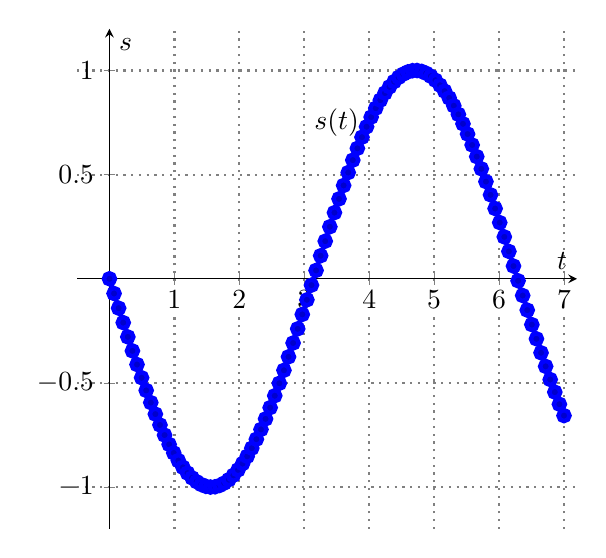
\begin{tikzpicture}
            \begin{axis}[axis x line=center, axis y line=middle,
            width=2.5in, height=2.5in, 
            scale only axis, %axis equal,
            xmin=-0.5, xmax=7.2,
            ymin=-1.2, ymax=1.2,
            xtick={0,...,7}, ytick={-1,-0.5,...,1},
            xticklabel style={draw=none, inner sep=2pt, fill=white, text opacity=1},
            xlabel={$t$}, ylabel={$s$},
            grid=both, grid style={line width=.8pt, draw=gray, dotted},
            minor tick num=0, 
            samples=100]
            \addplot+[blue, ultra thick, domain=0:7] {-sin(x*180/pi)};
            \node at (3.5, 0.75) {$s(t)$};
            \end{axis}
            \end{tikzpicture}
            \tinysp
            
            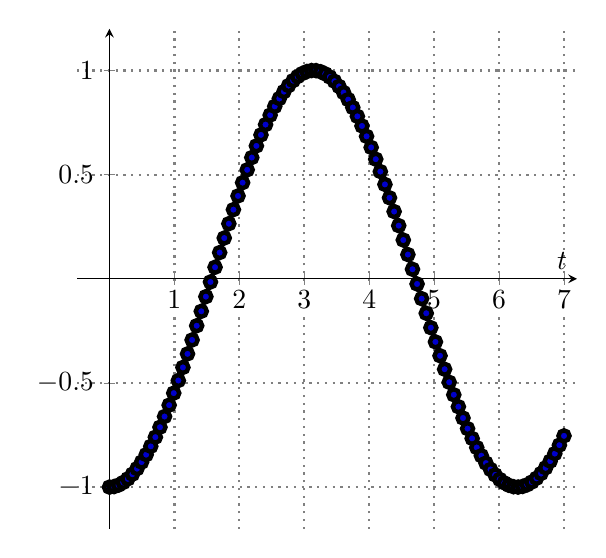
\begin{tikzpicture}
            \begin{axis}[axis x line=center, axis y line=middle,
            width=2.5in, height=2.5in, 
            scale only axis, %axis equal,
            xmin=-0.5, xmax=7.2,
            ymin=-1.2, ymax=1.2,
            xtick={0,...,7}, ytick={-1,-0.5,...,1},
            xticklabel style={draw=none, inner sep=2pt, fill=white, text opacity=1},
            xlabel={$t$}, ylabel={},
            grid=both, grid style={line width=.8pt, draw=gray, dotted},
            minor tick num=0, 
            samples=100]
            \addplot+[black, ultra thick, domain=0:7] {-cos(x*180/pi)};
            \end{axis}
            \end{tikzpicture}
            
            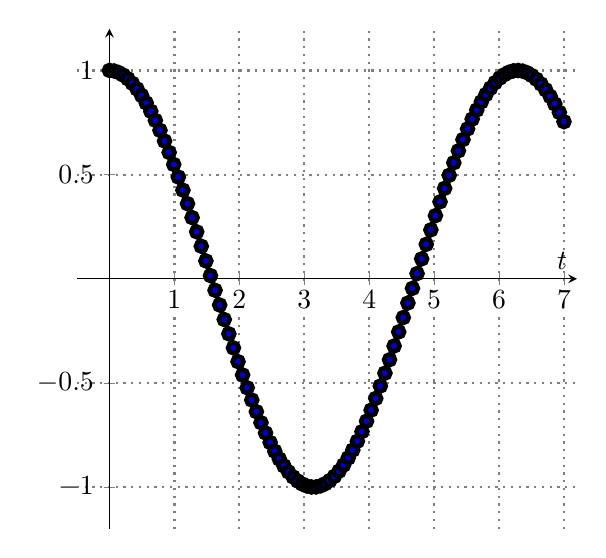
\begin{tikzpicture}
            \begin{axis}[axis x line=center, axis y line=middle,
            width=2.5in, height=2.5in, 
            scale only axis, %axis equal,
            xmin=-0.5, xmax=7.2,
            ymin=-1.2, ymax=1.2,
            xtick={0,...,7}, ytick={-1,-0.5,...,1},
            xticklabel style={draw=none, inner sep=2pt, fill=white, text opacity=1},
            xlabel={$t$}, ylabel={},
            grid=both, grid style={line width=.8pt, draw=gray, dotted},
            minor tick num=0, 
            samples=100]
            \addplot+[black, ultra thick, domain=0:7] {cos(x*180/pi)};
            \end{axis}
            \end{tikzpicture}
            \tinysp
            
            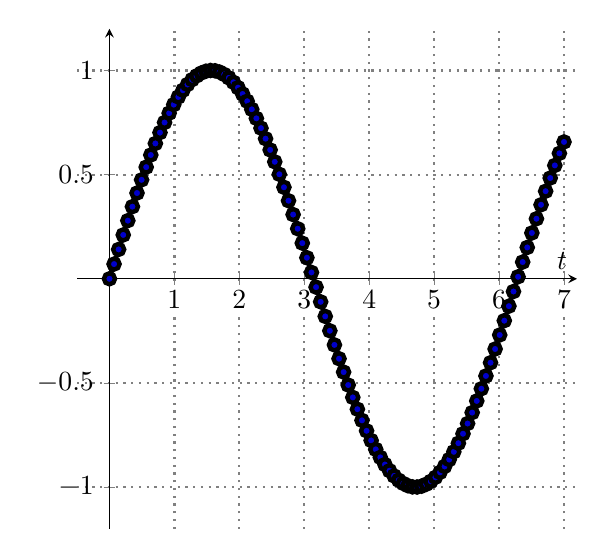
\begin{tikzpicture}
            \begin{axis}[axis x line=center, axis y line=middle,
            width=2.5in, height=2.5in, 
            scale only axis, %axis equal,
            xmin=-0.5, xmax=7.2,
            ymin=-1.2, ymax=1.2,
            xtick={0,...,7}, ytick={-1,-0.5,...,1},
            xticklabel style={draw=none, inner sep=2pt, fill=white, text opacity=1},
            xlabel={$t$}, ylabel={},
            grid=both, grid style={line width=.8pt, draw=gray, dotted},
            minor tick num=0, 
            samples=100]
            \addplot+[black, ultra thick, domain=0:7] {sin(x*180/pi)};
            \end{axis}
            \end{tikzpicture}
        \end{multicols}
    \end{multipartquestion}

    \frq{What is the derivative of $f(x)=x^2\cot(x)$?}
\end{document}